\documentclass[12pt]{article}
\usepackage[a4paper, top=0.8in, bottom=0.7in, left=0.8in, right=0.8in]{geometry}
\usepackage{amsmath}
\usepackage{amsfonts}
\usepackage{latexsym}
\usepackage{graphicx}
\usepackage{fancyhdr}
\usepackage{tcolorbox}
\usepackage{enumitem}
\usepackage{setspace}
\usepackage[defaultfam,tabular,lining]{montserrat} % Font settings for Montserrat
\usepackage{tikz} % For number line and visual tasks
\usepackage{xcolor} % For colored text

% General Comment: Template for creating problem sets aligned with a specific standard.

\setlength{\parindent}{0pt}
\pagestyle{fancy}

\setlength{\headheight}{27.11148pt}
\addtolength{\topmargin}{-15.11148pt}

\fancyhf{}
%\fancyhead[L]{\textbf{3.NF.A.1: Understanding Fractions as Numbers - Answer Key}} % Header with standards and topic title
\fancyhead[R]{
\includegraphics[width=0.8cm]{Round Logo.png}} % Placeholder for logo
\fancyfoot[C]{\footnotesize © Study Smart Tutors}

\sloppy

\newcommand{\dsfrac}[2]{\displaystyle\frac{#1}{#2}}

\title{}
\date{}
\hyphenpenalty=10000
\exhyphenpenalty=10000

\begin{document}

\subsection*{Problem Set: Understanding Fractions as Numbers - Answer Key}
\onehalfspacing

% Learning Objective Box
\begin{tcolorbox}[colframe=black!40, colback=gray!5, 
coltitle=black, colbacktitle=black!20, fonttitle=\bfseries\Large, 
title=Learning Objective, halign title=center, left=5pt, right=5pt, top=5pt, bottom=15pt]
\textbf{Objective:} Understand fractions as numbers by interpreting and representing fractions on number lines and visual models.
\end{tcolorbox}

% Exercises Box
\begin{tcolorbox}[colframe=black!60, colback=white, 
coltitle=black, colbacktitle=black!15, fonttitle=\bfseries\Large, 
title=Exercises, halign title=center, left=10pt, right=10pt, top=10pt, bottom=45pt]
\begin{enumerate}[itemsep=1.5em]
    \item Write the fraction that represents \(3\) shaded parts out of \(4\) total parts.\\
    \textcolor{red}{\textbf{Solution:} The fraction is \(\displaystyle \frac{3}{4}\).}

    \item Mark the fraction \(\displaystyle\frac{1}{2}\) on the number line below.  
    \begin{center}
        \begin{tikzpicture}[x=2cm, y=1cm]
            % Number line
            \draw[thick, ->] (0,0) -- (2,0);
            % Major ticks
            \foreach \x in {0,1,2} {
                \draw[thick] (\x,0.1) -- (\x,-0.1) node[below] {\x};
            }
            % Minor ticks
            \foreach \x in {0.5,1.5} {
                \draw[thick] (\x,0.05) -- (\x,-0.05);
            }
            % Mark solution
            \filldraw[red] (0.5,0) circle (3pt);
        \end{tikzpicture}
    \end{center}

    \item Write \(\displaystyle\frac{3}{6}\) in simplest form.\\
    \textcolor{red}{\textbf{Solution:} Simplify \(\displaystyle\frac{3}{6}\) by dividing numerator and denominator by their GCD (3): \(\displaystyle\frac{3}{6} = \frac{1}{2}\).}

    \item Divide the shape below into \(4\) equal parts. \\Shade \(3\) of them to represent \(\displaystyle \frac{3}{4}\).  
    \begin{center}
        \begin{tikzpicture}
            \draw[thick] (0,0) rectangle (4,2); % Draw rectangle
            \draw[thick] (1,0) -- (1,2); % Vertical lines
            \draw[thick] (2,0) -- (2,2);
            \draw[thick] (3,0) -- (3,2);
            \fill[red!30] (0,0) rectangle (3,2); % Shaded parts
        \end{tikzpicture}
    \end{center}

    \item Write the fraction represented by the point marked on the number line below.
    \begin{center}
        \begin{tikzpicture}[x=2cm, y=1cm]
            % Number line
            \draw[thick, ->] (0,0) -- (2,0);
            % Major ticks
            \foreach \x in {0,1,2} {
                \draw[thick] (\x,0.1) -- (\x,-0.1) node[below] {\x};
            }
            % Minor ticks
            \foreach \x in {.25, 0.5, .75, 1.25, 1.5, 1.75} {
                \draw[thick] (\x,0.05) -- (\x,-0.05);
            }
            % Mark fraction
            \filldraw[red] (1.5,0) circle (3.5pt)  ;
        \end{tikzpicture}
    \end{center}
    \textcolor{red}{\textbf{Solution:} The marked point is at \(1\frac{1}{2}\) or \(\displaystyle \frac{3}{2}\).}

    \item What fraction is equivalent to \(\displaystyle\frac{2}{4}\)? Write two examples.\\
    \textcolor{red}{\textbf{Solution:} Examples of equivalent fractions are \(\displaystyle \frac{1}{2}\) and \(\displaystyle \frac{4}{8}\).}

    \item Convert \(\displaystyle \frac{5}{10} \) to a decimal.\\
    \textcolor{red}{\textbf{Solution:} Divide 5 by 10: \(\displaystyle \frac{5}{10} = 0.5\).}

    \item Write the fraction that represents \(7\) shaded parts out of \(10\) total parts.\\
    \textcolor{red}{\textbf{Solution:} The fraction is \(\displaystyle \frac{7}{10}\).}
\end{enumerate}
\end{tcolorbox}

% Additional sections like Problems, Performance Task, and Reflection can follow the same pattern of adding red solutions.
\end{document}
